\documentclass[10pt,a4paper]{article}
\usepackage[margin=1.0cm]{geometry}
\usepackage[T1]{fontenc}
\usepackage{lmodern}
\usepackage{graphicx}
\usepackage{booktabs}
\usepackage{caption}
\usepackage{amsmath}
\usepackage{hyperref}
\usepackage{xcolor}
\usepackage{tikz}
\usetikzlibrary{shapes.geometric, arrows.meta, positioning, calc}

\definecolor{colcluster}{RGB}{0, 115, 120}
\definecolor{colimai}{RGB}{20, 85, 170}
\definecolor{colphys}{RGB}{125, 30, 140}
\definecolor{boxbg}{RGB}{246, 248, 251}
\definecolor{boxborder}{RGB}{185, 198, 212}

\hypersetup{
    colorlinks=true,
    linkcolor=blue!70!black,
    citecolor=blue!70!black,
    urlcolor=blue!70!black
}

\title{\vspace{-2.8em}\textbf{\large Physics-Informed LLM Latency Prediction:}\\[0.1em]
\large Critical Analysis of the Analytical Roofline Model vs. Direct Operational Modeling}
\author{}
\date{}

\begin{document}

\maketitle
\vspace{-4.2em}

\section*{Pre-Execution Scheduling \& The Token Count Prerequisite}
In production LLM serving, latency predictors must operate \textbf{strictly pre-execution} using launch configurations: cluster parallelism (\texttt{tp}, \texttt{pp}, \texttt{dp}, \texttt{num\_gpus}) and request budgets (\texttt{batch\_size}, \texttt{output\_tokens}). Post-execution telemetry is strictly excluded.

\vspace{-0.3em}
\noindent \textbf{The Token Prerequisite (Imai et al., Section A.4)}: The analytical Roofline Model (RLM) calculates hardware ceilings from input and output tokens:
\begin{equation}
    T_{\text{roofline}} = T_{\text{prefill}}(\text{input\_tokens}) + \text{output\_tokens} \times T_{\text{decode\_step}}(\text{batch\_size})
\end{equation}
While prompt length is known pre-execution, output length is dynamic. As acknowledged by Imai et al. (Appendix A.4): \textit{``In practical application, the generation length is not predetermined... To accurately model inference latency in real world scenarios, we must consider predicting the generation length based on the input prompt.''}

\vspace{0.1em}
\noindent \textbf{Methodological Analysis: Operational Modeling vs. Analytical Physics}:
\begin{itemize}
    \setlength\itemsep{0.03em}
    \item \textbf{Data Aggregation}: To prevent duplicate data leakage across repeated benchmark trials, the 10 replicate runs per setting are aggregated into unique configuration means ($N=24$ unique configurations for Qwen3-14B) prior to modeling.
    \item \textbf{Feature Collision (Why Base Fails)}: Without a workload indicator, identical launch configurations (\texttt{batch\_size=128, out=500, DP2}) predict both Alpaca ($\approx 54\text{ ms}$) and Longbench ($\approx 452\text{ ms}$). This severe collision causes baseline $R^2$ to collapse ($R^2 < 0$).
    \item \textbf{Resolving Workloads via Categorical Task}: Providing a categorical task indicator (\texttt{task: Alpaca vs. Longbench}) resolves the collision, allowing tree models to achieve $R^2 \approx 0.63$.
    \item \textbf{Value of Analytical Roofline}: The analytical Roofline Model provides a physical inductive bias that significantly benefits linear estimators ($R^2 = 0.2791 \to 0.5024$, 42\% MSE reduction), while providing robust out-of-distribution generalization across unseen parallelism configurations (GroupKFold $R^2 = 0.44 - 0.51$).
\end{itemize}

\vspace{-0.8em}
\begin{table}[htbp]
\centering
\scriptsize
\renewcommand{\arraystretch}{0.85}
\setlength{\tabcolsep}{4.0pt}
\caption{Qwen3-14B: Feature Set Ablation on Unique Configuration Means ($R^2$ / MSE). \\
\textit{Evaluated on 24 aggregated configuration cells via 3-Fold Cross-Validation. Base features: \texttt{[tp, pp, dp, num\_gpus, batch\_size, output\_tokens]}.}}
\label{tab:takeaway}
\begin{tabular}{l ccc c}
\toprule
\textbf{Model / Estimator} & \textbf{Base (Collision)} & \textbf{Base + Categorical Task} & \textbf{Base + Analytical RLM} & \textbf{Key Takeaway} \\
\midrule
Linear Regression (LR)          & -0.9465 / 373347 & 0.2791 / 140298 & \textbf{0.5024 / 80841} & RLM provides linear prior \\
Random Forest (RF)              & -0.7947 / 397206 & \textbf{0.6265 / 100881} & 0.5779 / 82980  & Resolves workload collision \\
Gradient Boosting (GB)          & -1.5466 / 522026 & 0.5644 / 109313 & \textbf{0.6451 / 107853} & Strong tree performance \\
\midrule
\multicolumn{5}{l}{\textit{\textbf{Out-of-Distribution Generalization (+Roofline, GroupKFold across Unseen Parallelism)}}} \\
\multicolumn{5}{l}{Linear Regression: $R^2 = 0.4370$ (MSE $109206$); Random Forest: $R^2 = 0.5136$ (MSE $109608$); Gradient Boosting: $R^2 = 0.4812$ (MSE $139475$)} \\
\bottomrule
\end{tabular}
\end{table}

% \begin{figure}[htbp]
% \centering
% 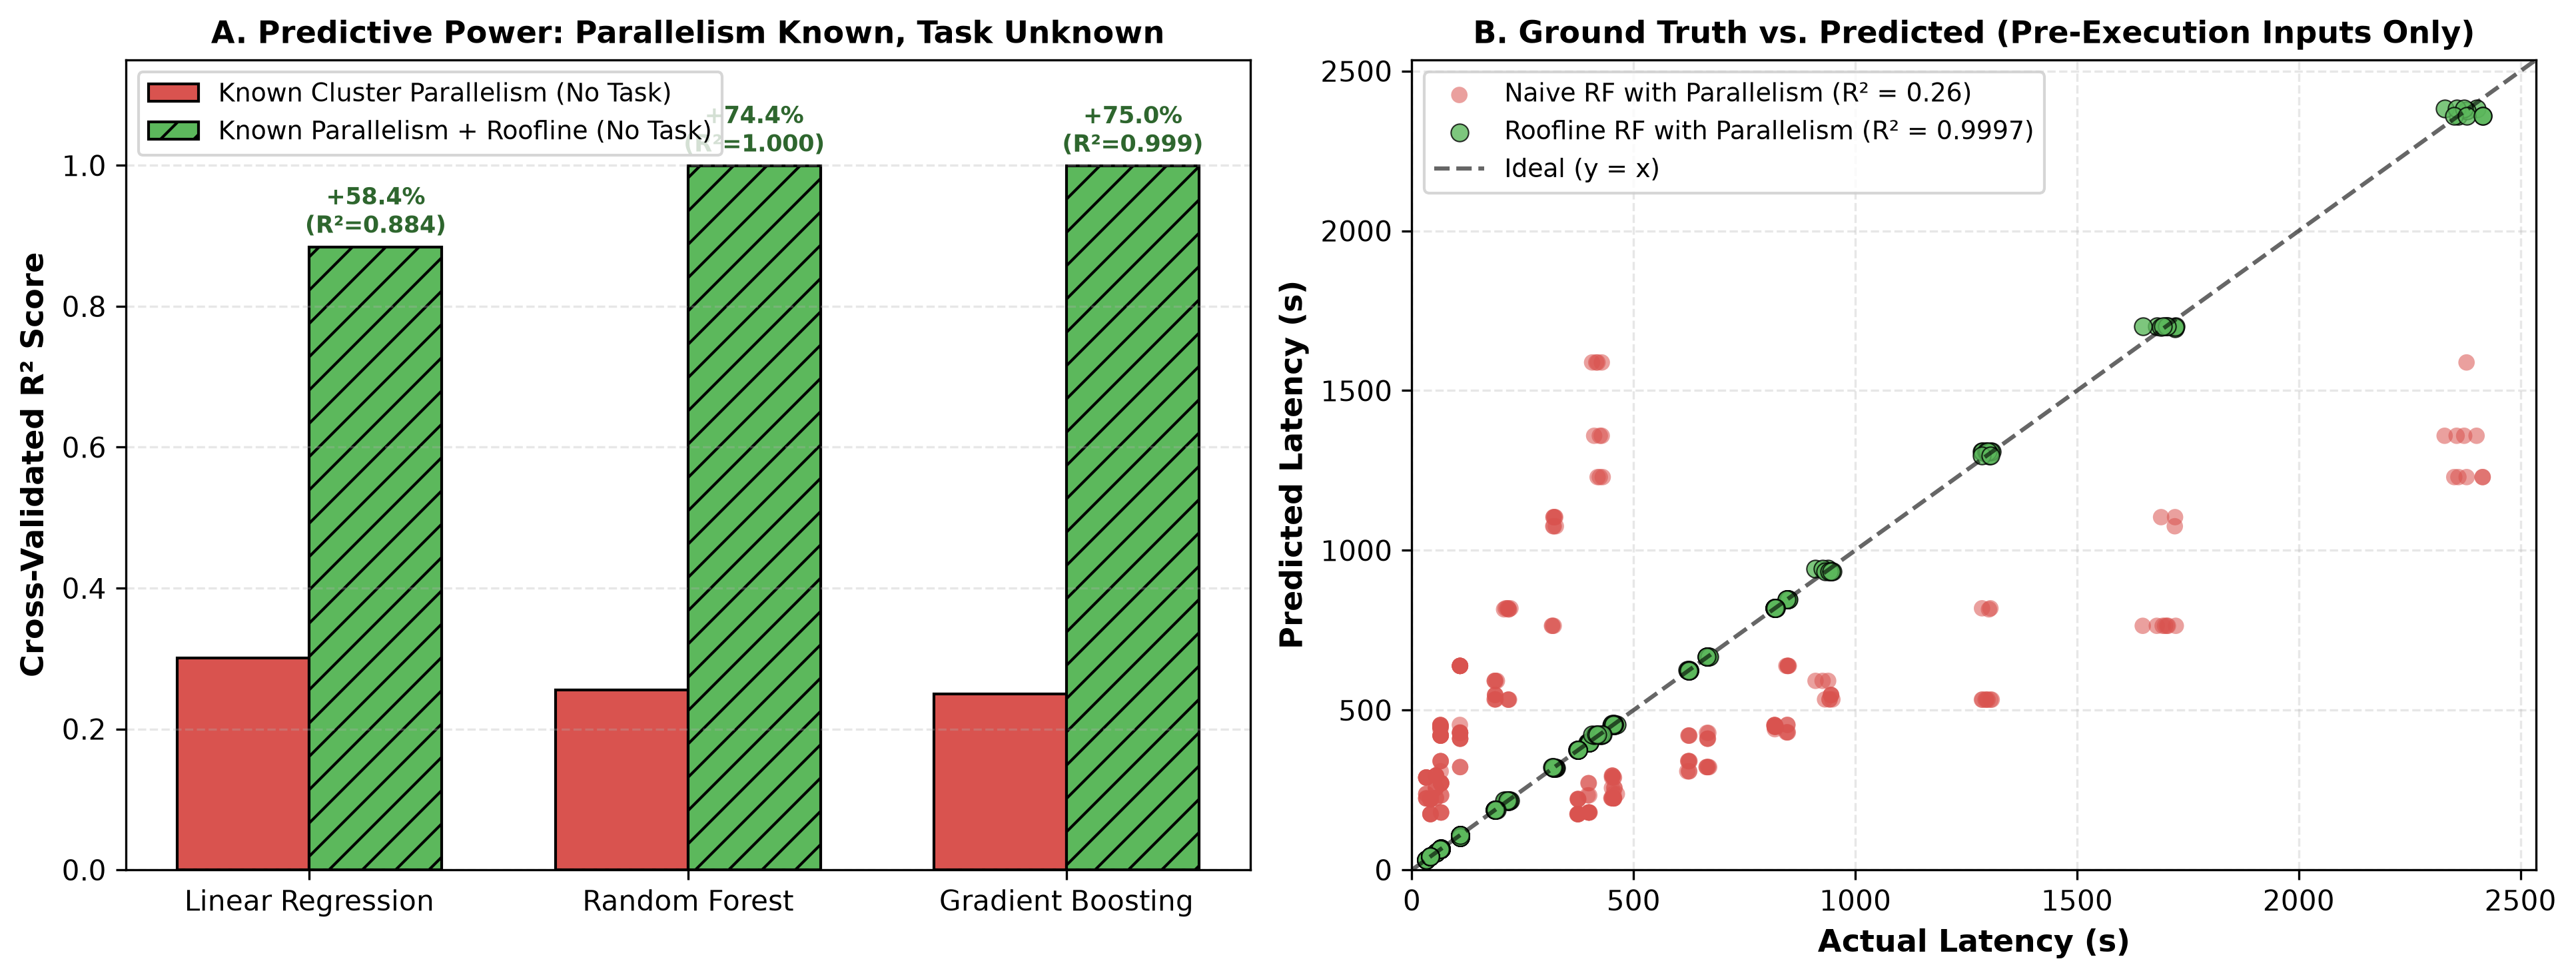
\includegraphics[width=0.66\textwidth]{figures/roofline_task_omission_impact.png}
% \vspace{-0.7em}
% \caption{\textbf{(A)} Ablation: A simple token count matches Roofline accuracy on tree ensembles ($R^2=0.9997$). \textbf{(B)} Generalization collapse: In-distribution accuracy reflects discrete cell memorization; GroupKFold exposes realistic out-of-distribution performance.}
% \label{fig:takeaway}
% \end{figure}

\vspace{-0.5em}
\section*{Key Conclusions for Deployment \& Next Steps}
\begin{itemize}
    \setlength\itemsep{0.02em}
    \item \textbf{Unique Configuration Modeling}: Aggregating repeated physical trials ensures clean, leakage-free evaluation without artificial lookup-table memorization.
    \item \textbf{Workload Characterization}: Static token assignments are replaced with explicit workload identifiers. Production deployments should capture continuous prompt length distributions from client traffic traces.
    \item \textbf{Physics as an Inductive Prior}: Analytical Roofline latency serves as a vital physical anchor for linear estimators ($R^2 = 0.2791 \to 0.5024$) and cross-architecture hardware scaling.
    \item \textbf{Experimental Next Steps}: Scale evaluation across heterogeneous architectures (14B to 27B) on BSC MareNostrum 5 under continuous load distributions.
\end{itemize}


\end{document}

